\def\retinafocusidea{
    Lấy cảm hứng từ hai mô hình RetinaFace \cite{deng2020retinaface} và AutoFocus \cite{najibi2019autofocus}, mô hình RetinaFocus được xây dựng nhằm tận dụng điểm mạnh và khắc phục điểm yếu của cả hai mô hình trên trong một mô hình duy nhất, từ đó, giải quyết tốt bài toán face detection trong ảnh chất lượng cao.

    \noindent
    \textbf{\textit{Ý tưởng chính của mô hình RetinaFocus}} \\
    Mô hình RetinaFace, như đã thảo luận ở \textbf{\textit{phần 4.2. Mô hình RetinaFace}}, là một mô hình có đạt độ chính xác tương đối cao trên bộ dữ liệu WIDER FACE cùng với tốc độ xử lý đạt mức chấp nhận được.
    Mặc dù sử dụng FPN trong kiến trúc backbone của mình, mô hình RetinaFace vẫn chưa thể dự đoán với vị trí bbox chính xác và với độ tự tin cao hết những mặt có kích thước nhỏ.
    Do đó, khi xử lý ảnh có kích thước lớn, để duy trì được độ chính xác cao, nhóm tác giả vẫn sử dụng chiến lược Image Pyramids và điều đó khiến cho tốc độ xử lý của RetinaFace tăng lên nhiều lần. \\
    Bên cạnh đó, mô hình AutoFocus, như đã thảo luận ở \textbf{\textit{phần 3.4. Mô hình AutoFocus}}, lại là một giải pháp rất thông minh để xử lý ảnh với chiến lược Image Pyramids nhưng với tốc độ cao và chi phí tính toán thấp. \\
    Từ những điểm yếu của mô hình RetinaFace khi xử lý ảnh chất lượng cao và những điểm mạnh của mô hình AutoFocus, chúng tôi đề xuất mô hình RetinaFocus giải bài toán face detection trong ảnh chất lượng cao với độ chính xác tương đương và cải thiện đáng kể tốc độ tính toán.

    \noindent
    \textbf{\textit{Kiến trúc mô hình RetinaFocus}} \\
    Kiến trúc mô hình RetinaFocus lấy mô hình RetinaFace làm nền tảng, kết hợp cùng nhánh Focus của mô hình AutoFocus.
    Nói cách khác, mô hình RetinaFace được sử dụng để thay thế cho mô hình Faster R-CNN của nhánh detection trong mô hình AutoFocus.
    Cụ thể hơn, một trong số các feature maps được trích xuất từ backbone FPN, bên cạnh việc được qua các Context Module như trong mô hình RetinaFace nguyên bản, còn được đưa qua các lớp Conv của nhánh Focus giúp xác định được khu vực đáng chú ý trên ảnh và loại bỏ các khu vực khả năng cao không chứa khuôn mặt.

    \begin{figure}[H]
        \centering
        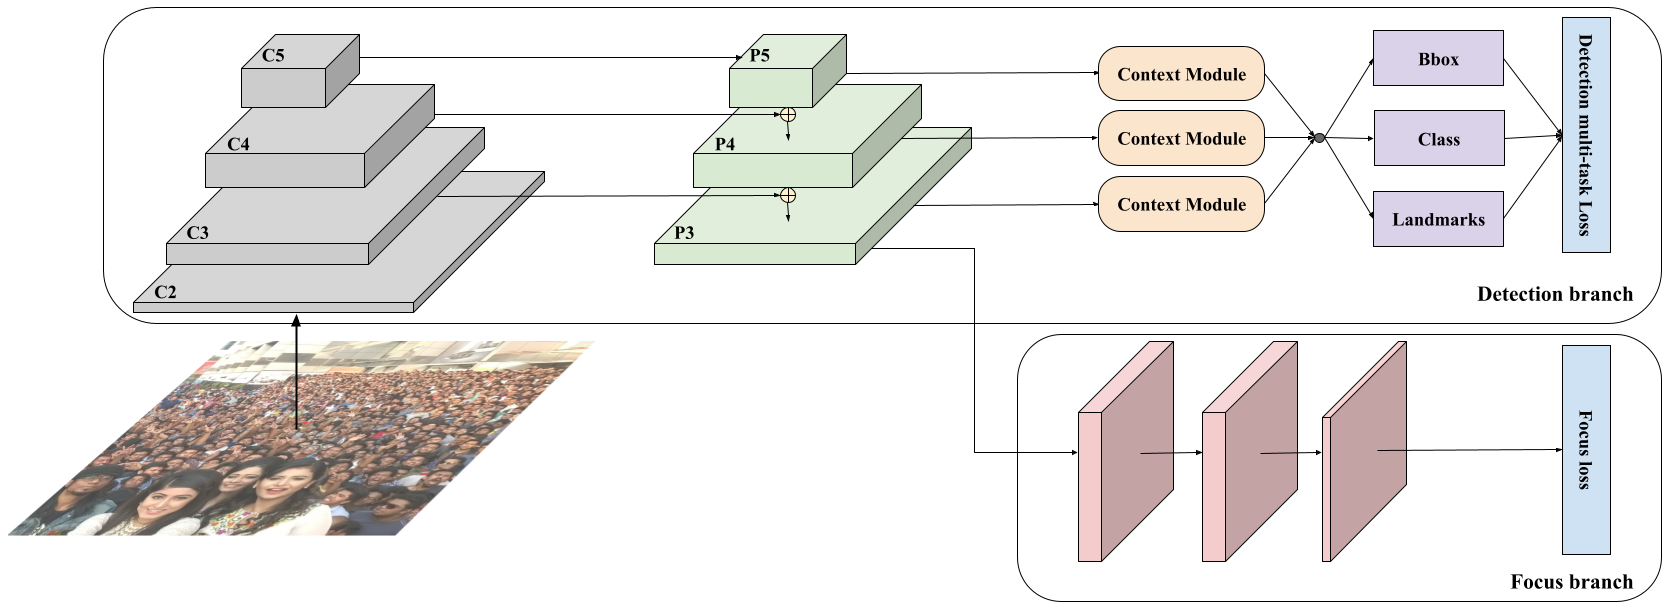
\includegraphics[width=10cm] {images/retinafocus_architecture}
        \caption{Kiến trúc của mô hình RetinaFace. (Nguồn: \cite{deng2020retinaface})}
        \label{fig:retinafocus_architecture}
    \end{figure}

    \noindent
    Hình trên là một ví dụ về kiến trúc mô hình RetinaFocus khi sử dụng feature maps P3 của FPN làm đầu vào cho nhánh Focus.
    Các feature maps khác của FPN cũng đều có thể được sử dụng làm đầu vào cho nhánh Focus và kết quả so sánh độ hiệu quả của các feature maps này sẽ được bàn luận kỹ hơn ở phần dưới. \\
    Đối với nhánh Detection của RetinaFocus, đầu ra được giữ nguyên so với mô hình RetinaFace nguyên bản gồm toạ độ của bounding box dự đoán của mô hình, toạ độ của landmarks của khuôn mặt và xác suất mà bounding box dự đoán đó chứa khuôn mặt.
    Các đầu ra này của nhánh Detection, sau đó, tiếp tục được đưa vào hàm loss multi-task, tương tự như mô hình RetinaFace. \\
    Đối với nhánh Focus của RetinaFocus, đầu ra vẫn là mask mà mô hình dự đoán và được đưa vào hàm loss để so sánh với mask gồm các giá trị -1, 0, 1 được sinh ra từ thuật toán Focus Pixel của mô hình AutoFocus.

    \noindent
    \textbf{\textit{Chuẩn bị dữ liệu cho nhánh Focus của mô hình}} \\
    Như đã thảo luận ở \textbf{\textit{phần 3.4}}, để sử dụng mô hình AutoFocus một cách hiệu quả, ta cần xây dựng được bộ tham số yêu cầu cho Thuật toán Focus Pixel, cụ thể là ba tham số $a, b, c$, đặc biệt là hai tham số $a$ và $b$ giúp định nghĩa ra khoảng kích thước bounding box cần được focus.
    Để xây dựng được bộ tham số này, ta cần phân tích điểm yếu của nhánh detection (cụ thể chính là mô hình RetinaFace) trên bộ dữ liệu WIDER FACE.
    Từ những điểm yếu, ta lựa chọn bộ tham số của nhánh Focus nhằm giúp cho nhánh focus xác định được những vùng mà nhánh detection dự đoán yếu và zoom vào giúp nhánh detection dự đoán chính xác hơn.

    \begin{figure}[H]
        \centering
        \subfigure[]{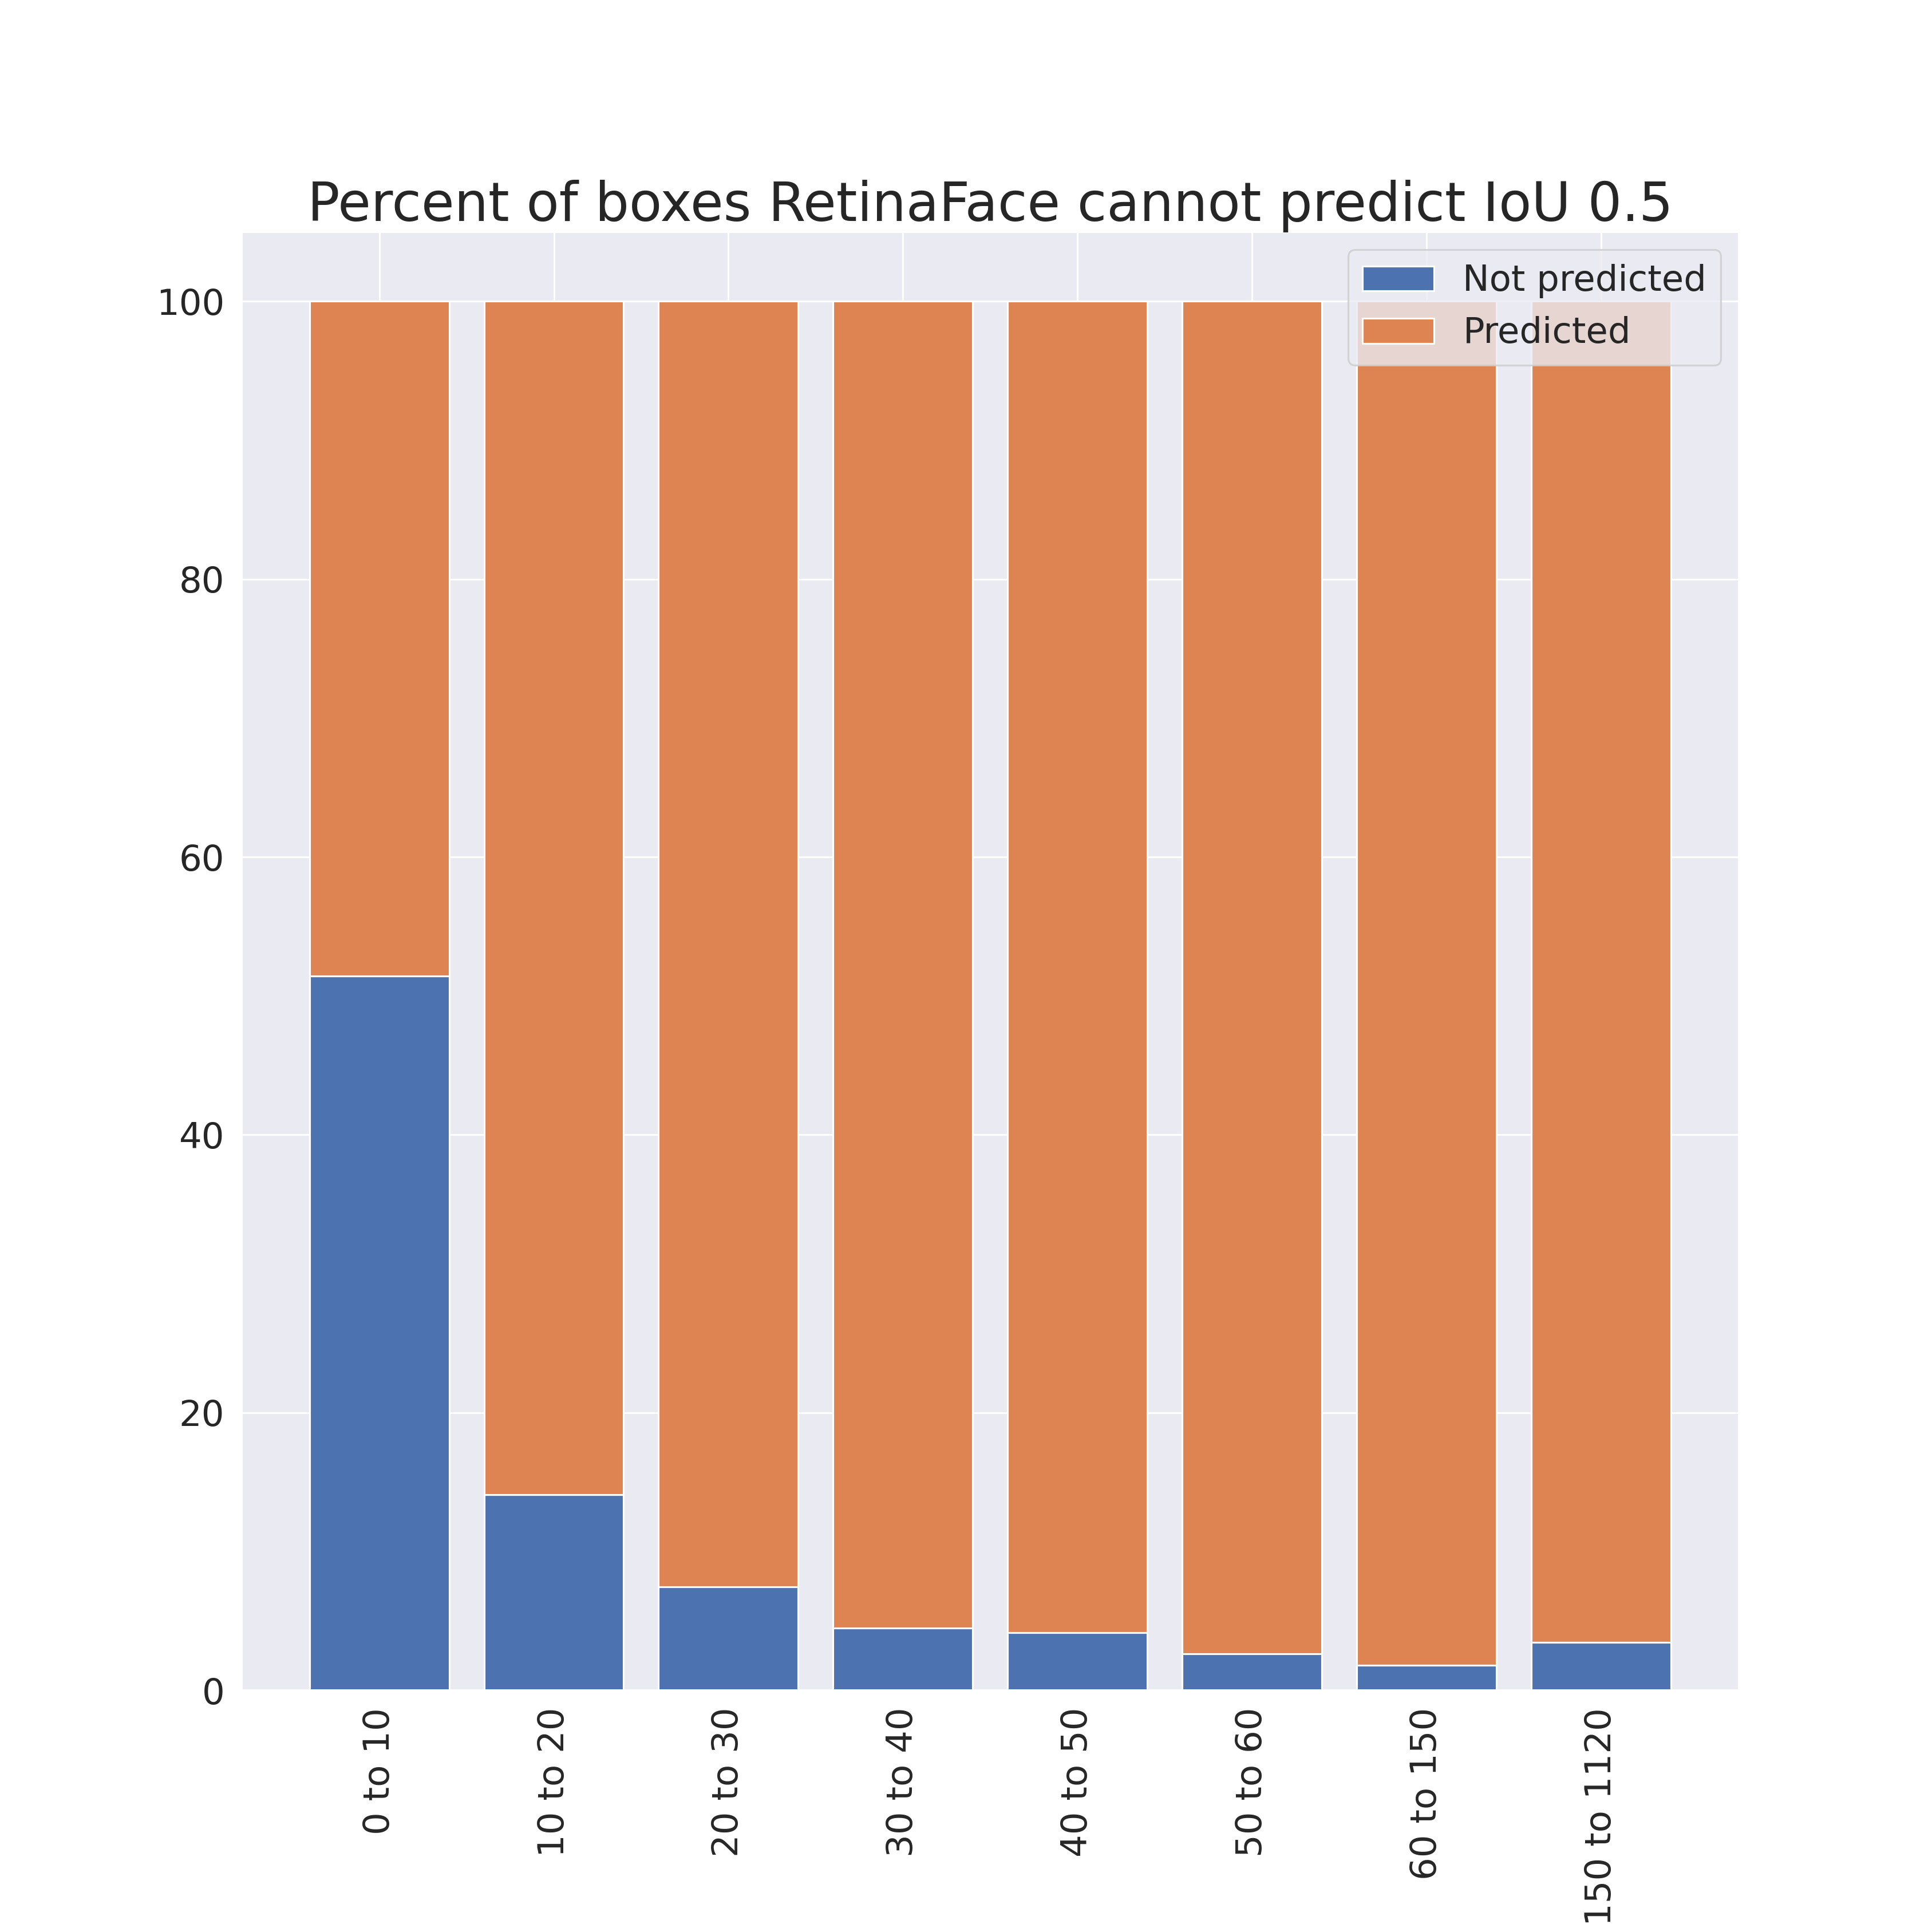
\includegraphics[width=0.32\textwidth, trim={2.3cm 2.3cm 2.3cm 2.3cm}, clip]{images/retinafocus_iou_50_compare_percent}} 
        \subfigure[]{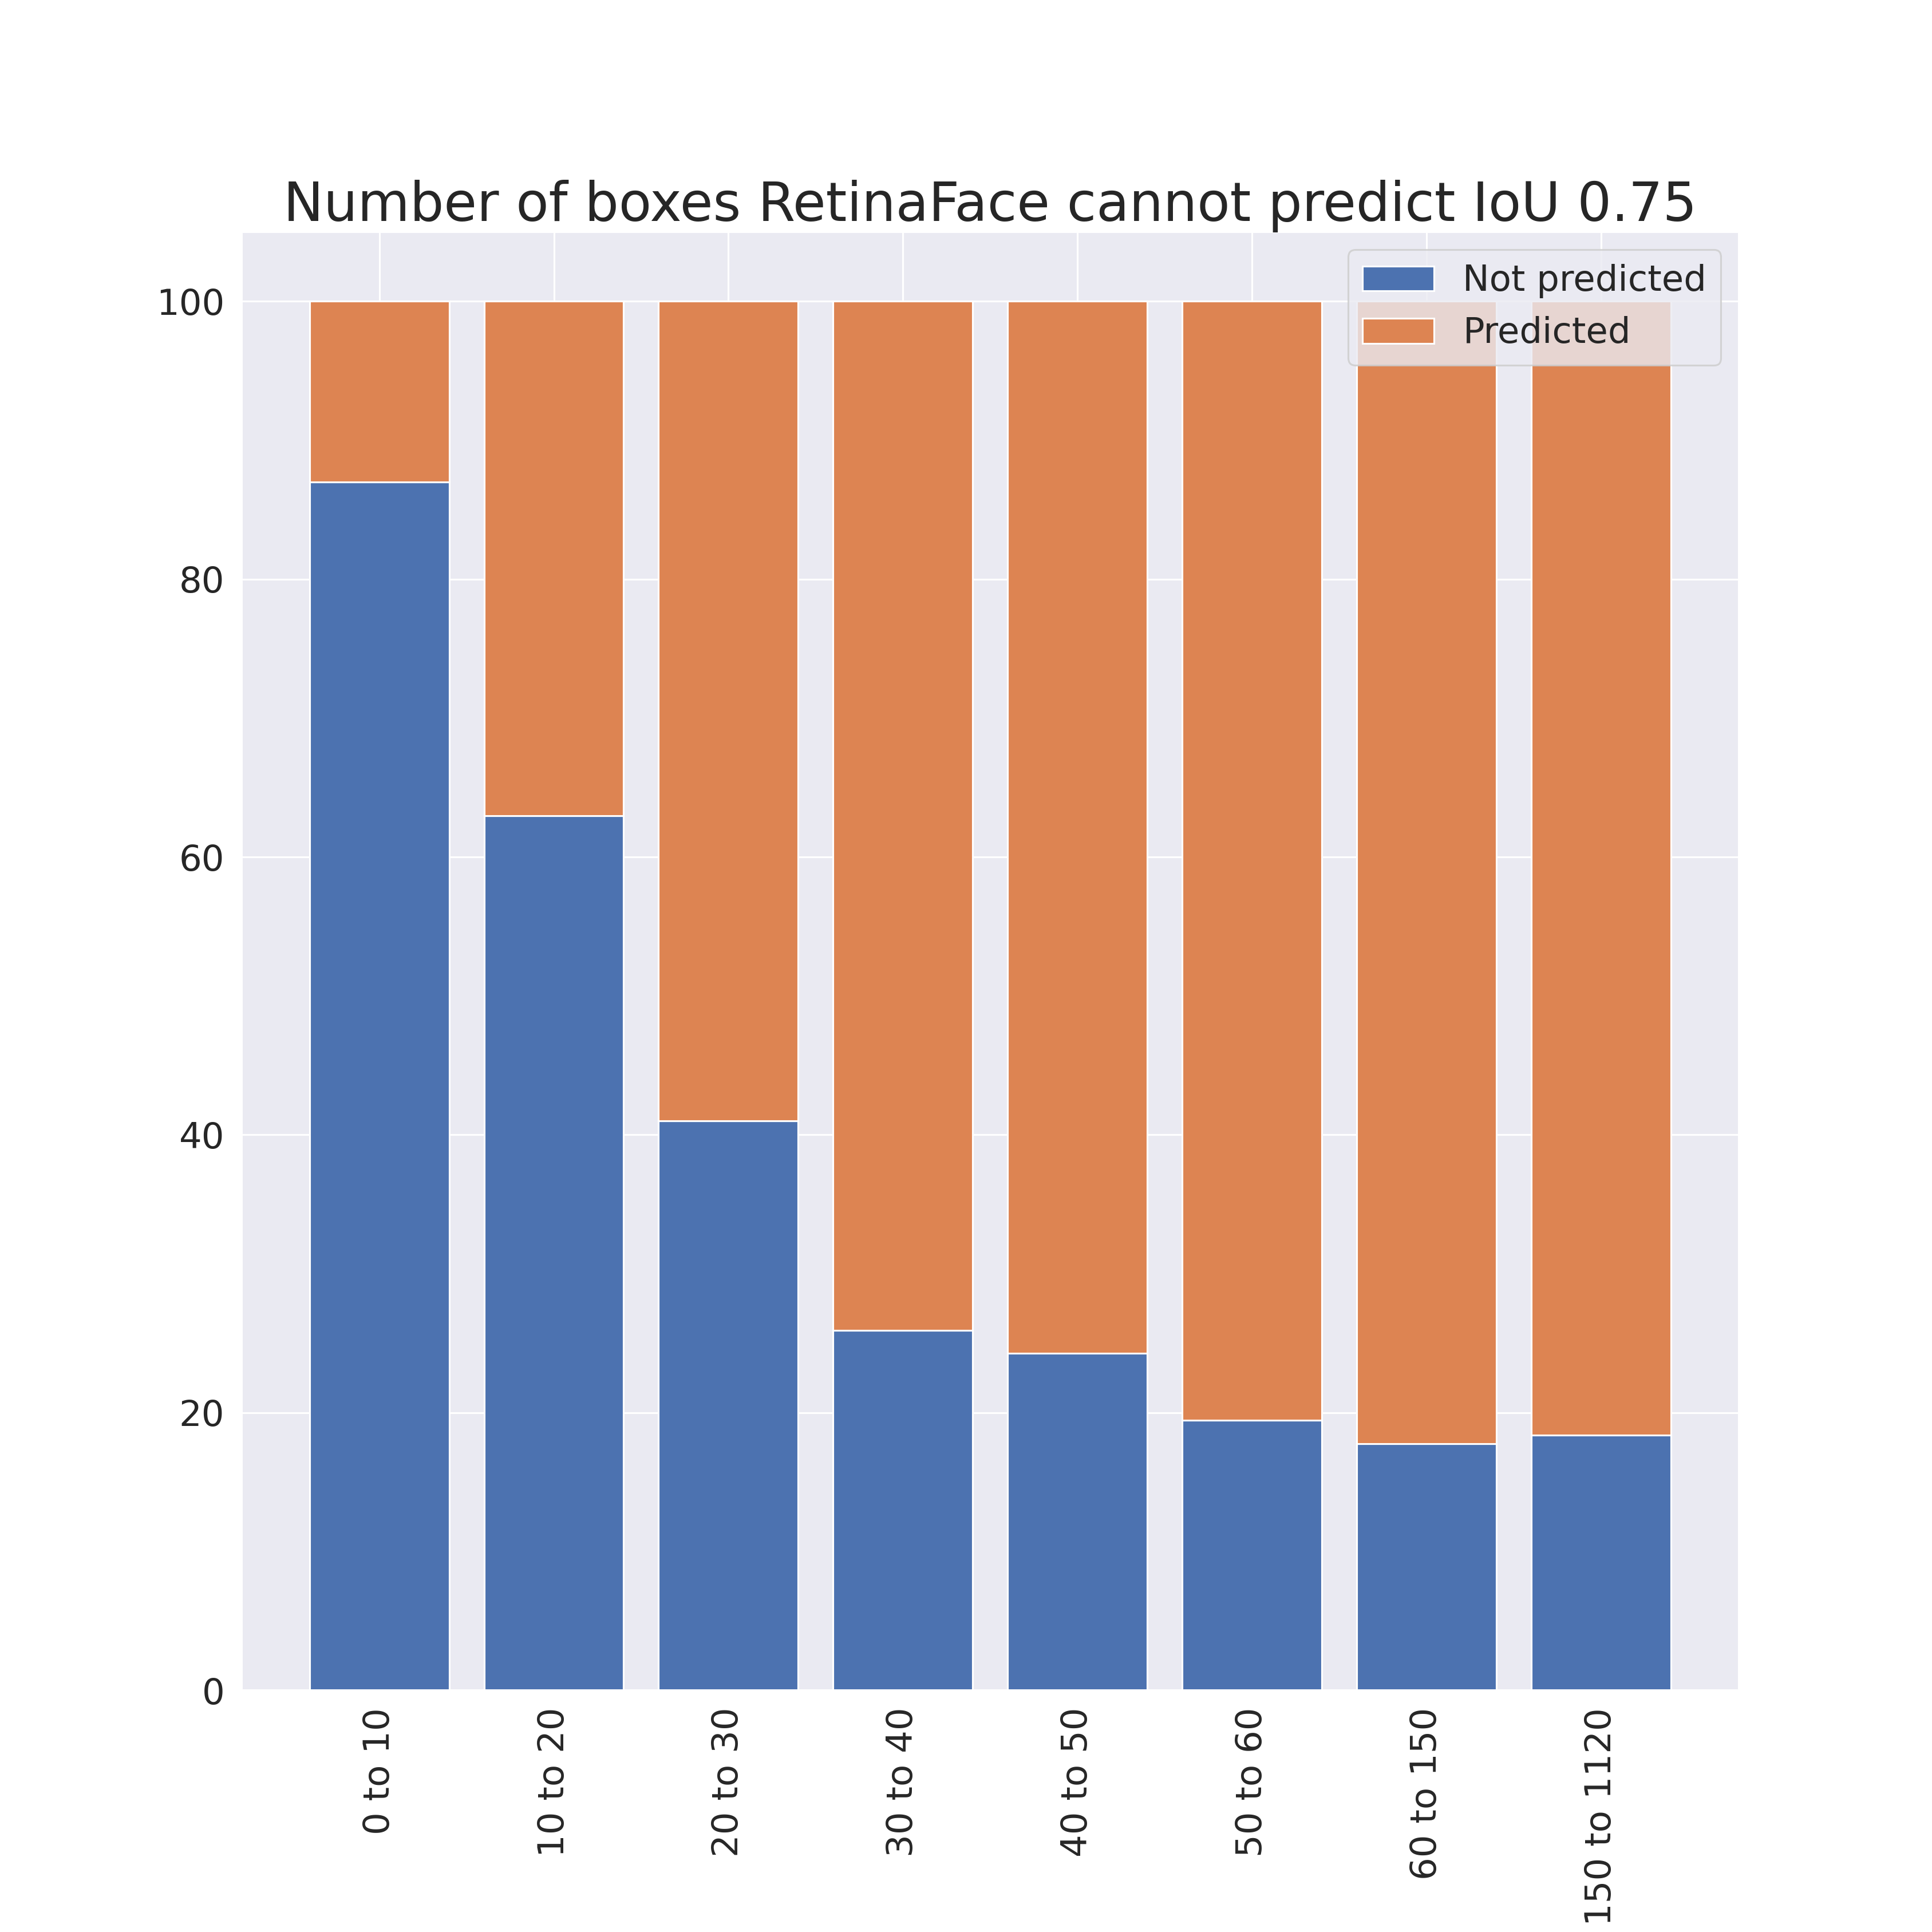
\includegraphics[width=0.32\textwidth, trim={2.3cm 2.3cm 2.3cm 2.3cm}, clip]{images/retinafocus_iou_75_compare_percent}} 
        \subfigure[]{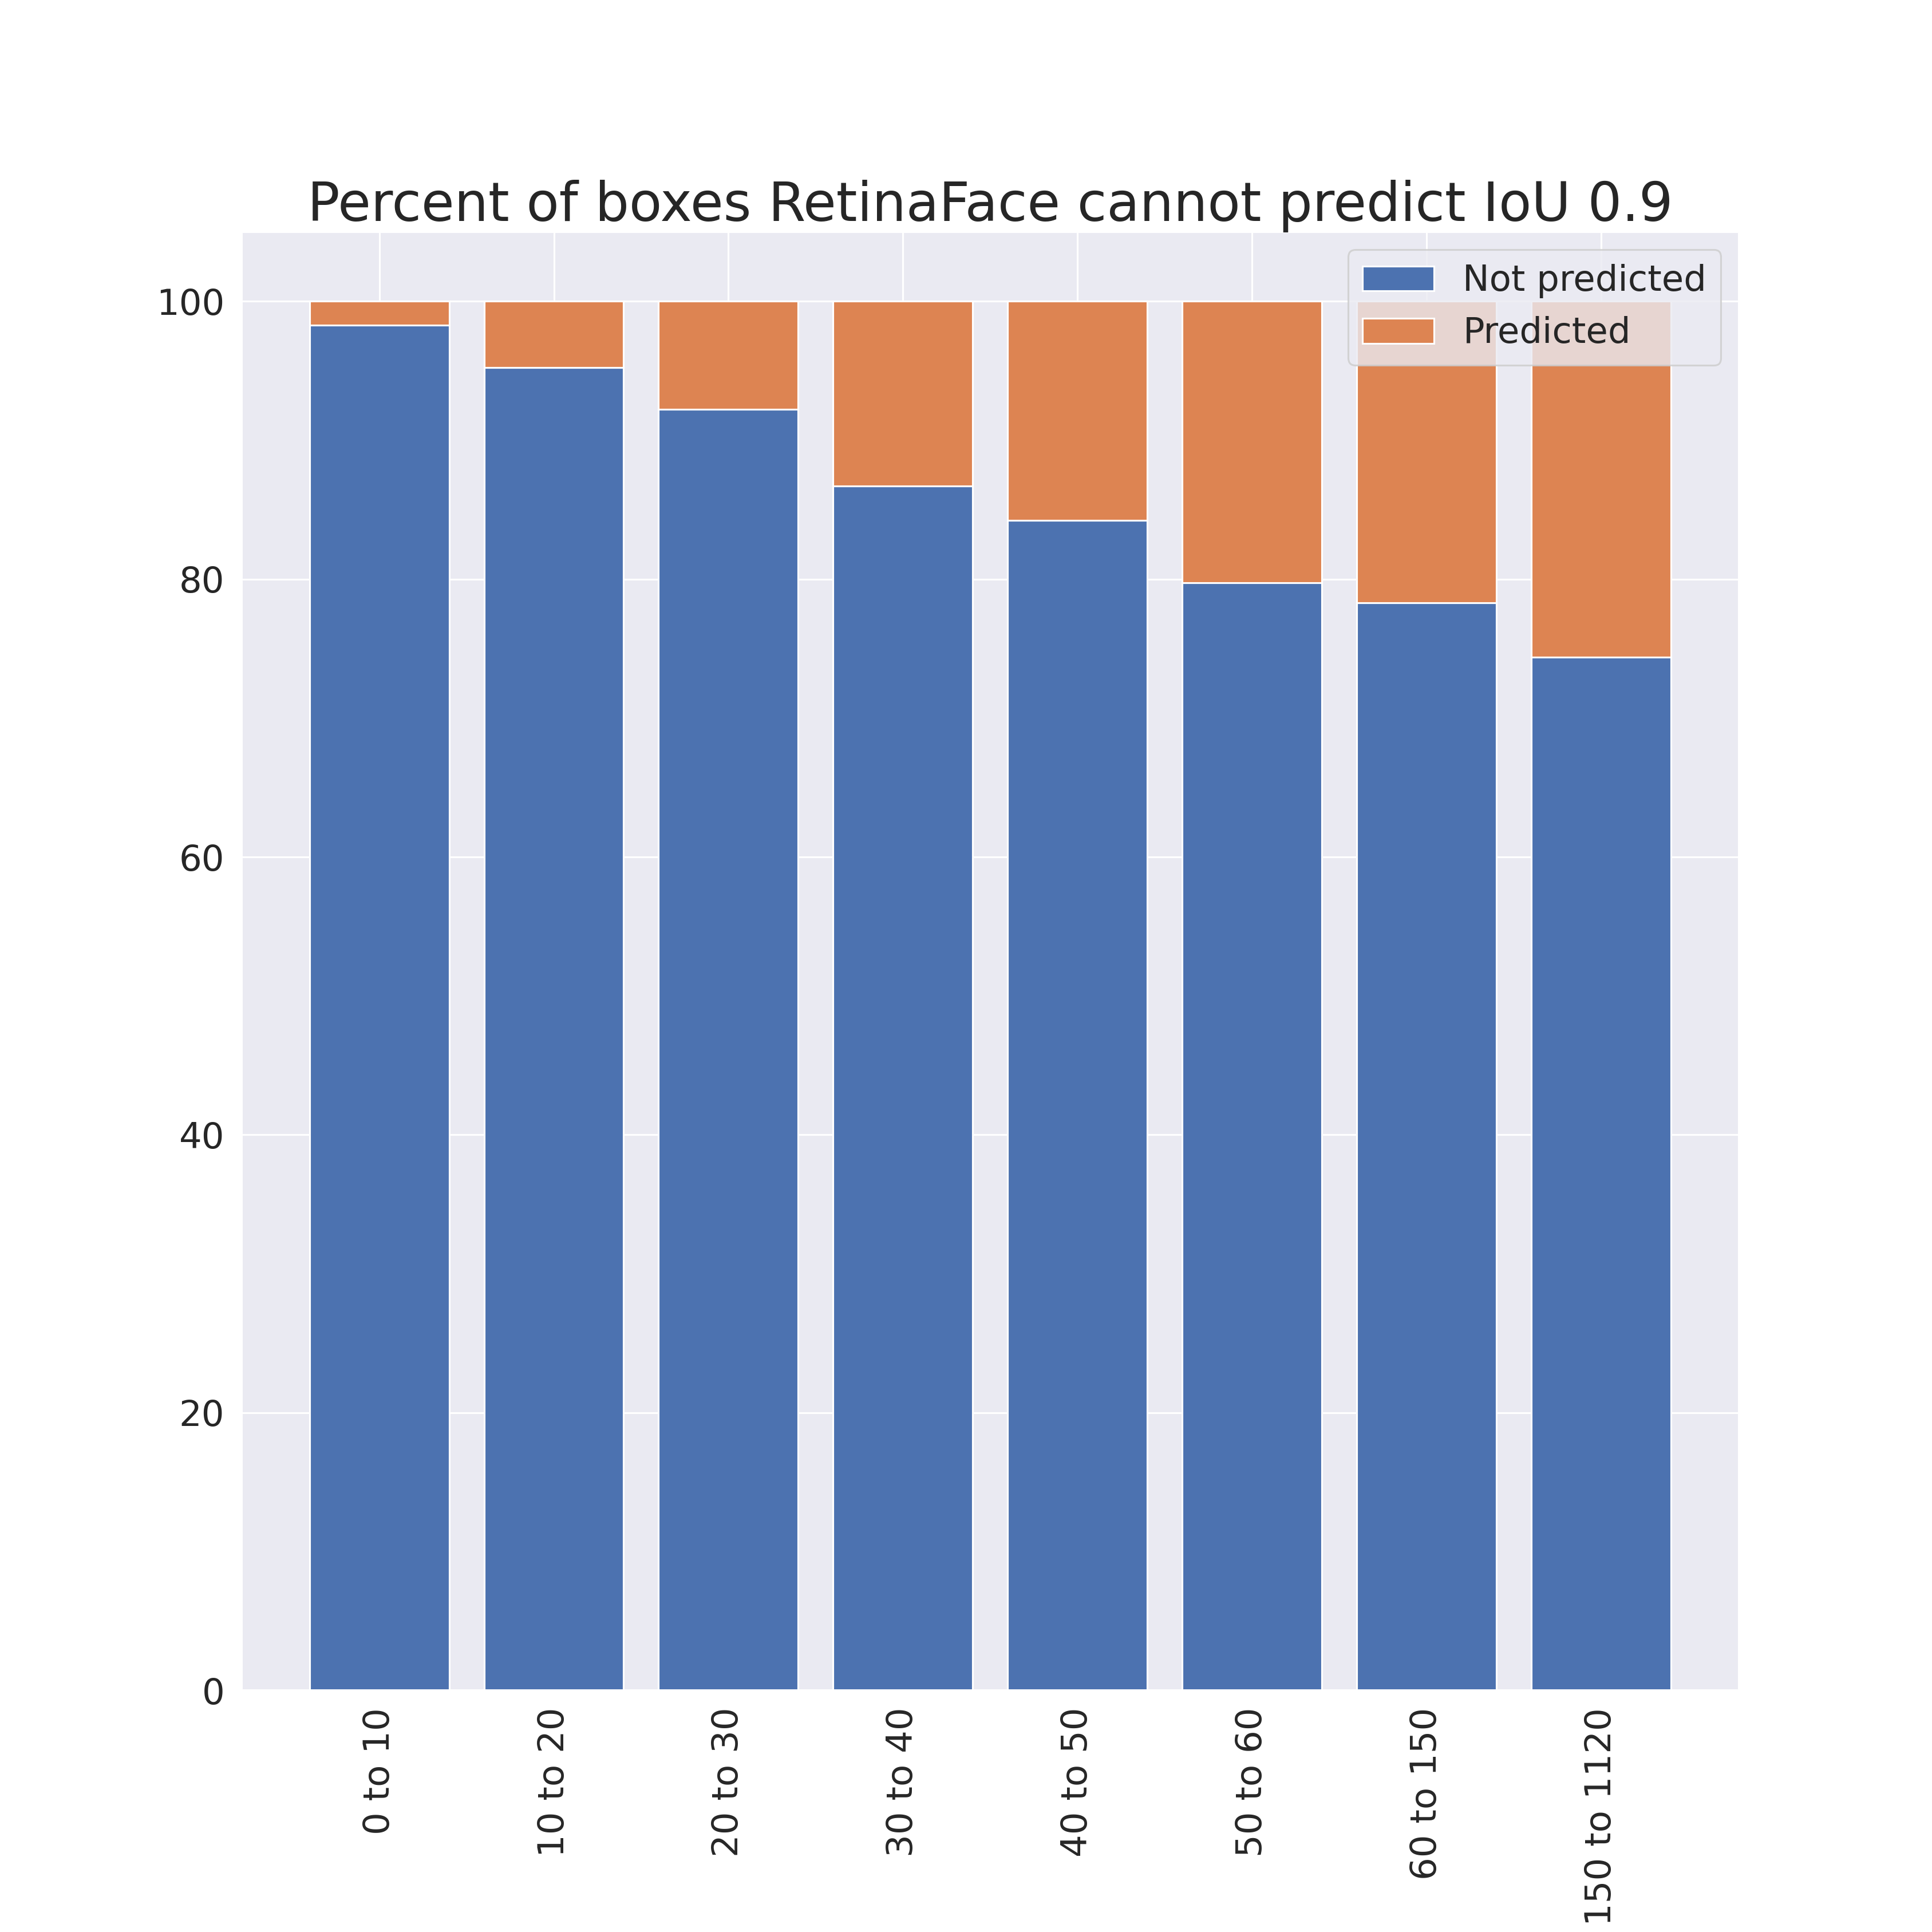
\includegraphics[width=0.32\textwidth, trim={2.3cm 2.3cm 2.3cm 2.3cm}, clip]{images/retinafocus_iou_90_compare_percent}} 
        \caption{Tỷ lệ số lượng bounding box mà mô hình RetinaFace dự đoán ra và không dự đoán ra tương ứng với IoU 0.5 (a), IoU 0.75 (b), IoU 0.9 (c)}
        \label{fig:retinafocus_iou_compare_percent}
    \end{figure}

    \noindent
    Trong hình \ref{fig:retinafocus_iou_compare_percent}, trên cả ba mức IoU, tỷ lệ số lượng bounding box mà mô hình RetinaFace không dự đoán ra đối với nhóm các bounding box nhỏ từ 0 pixel đến 30 pixel và đặc biệt là từ 0 pixel đến 10 pixel đều cao vượt trội so với các kích thước bounding box khác.

    \begin{figure}[H]
        \centering
        \subfigure[]{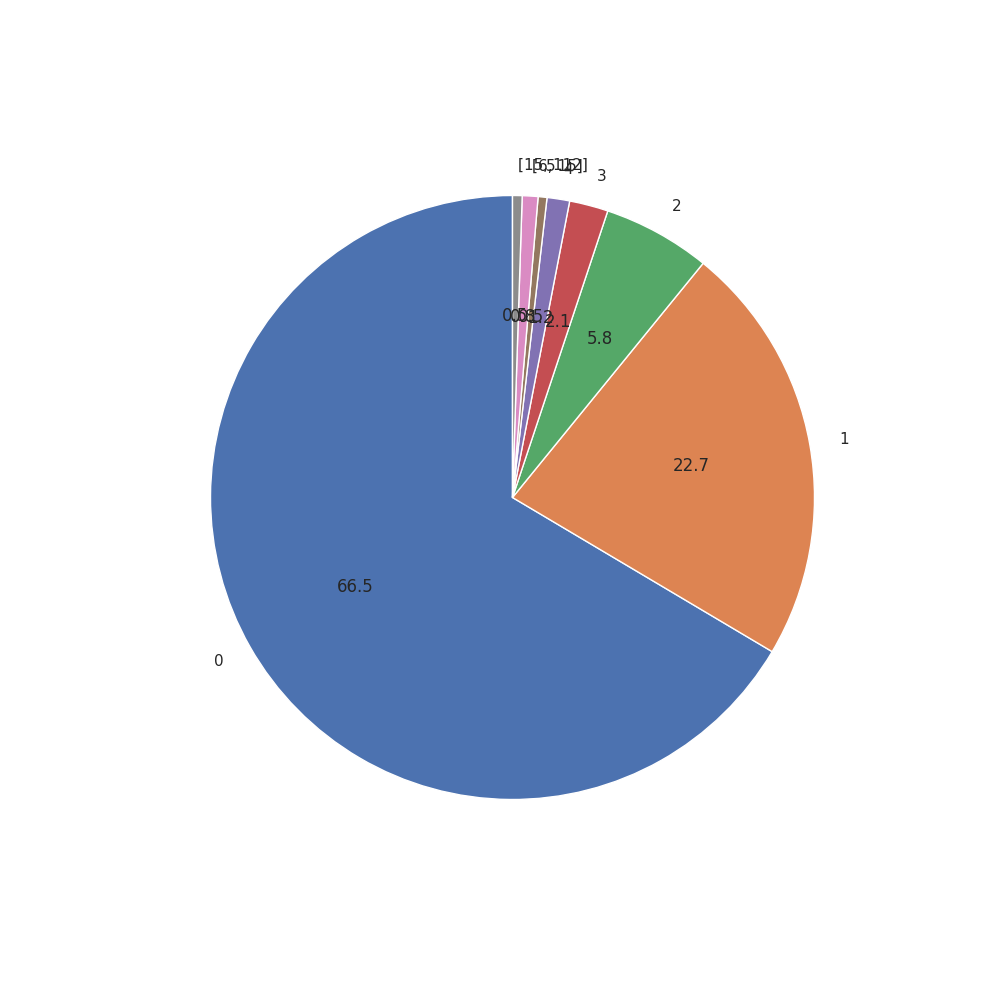
\includegraphics[width=0.32\textwidth, trim={5cm 4.7cm 4.3cm 4.6cm}, clip]{images/retinafocus_iou_50_lower}} 
        \subfigure[]{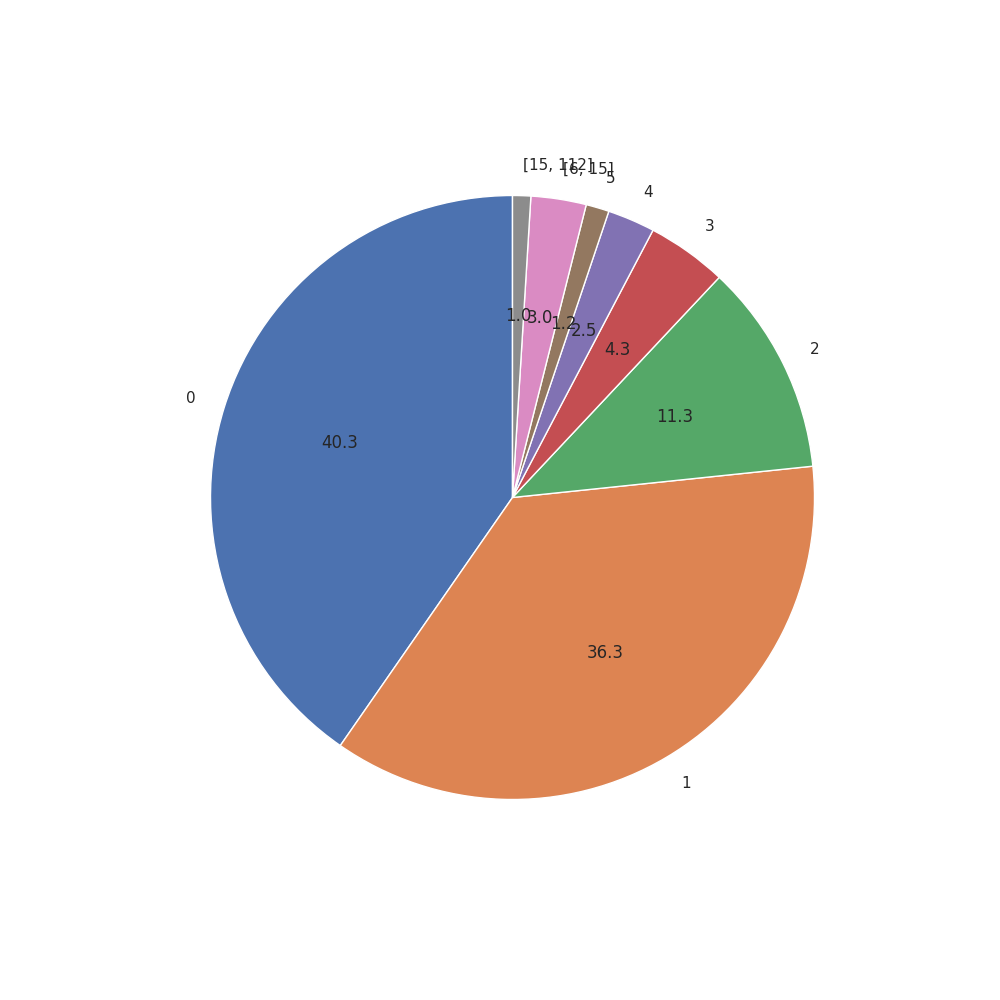
\includegraphics[width=0.32\textwidth, trim={5cm 4.7cm 4.3cm 4.6cm}, clip]{images/retinafocus_iou_75_lower}} 
        \subfigure[]{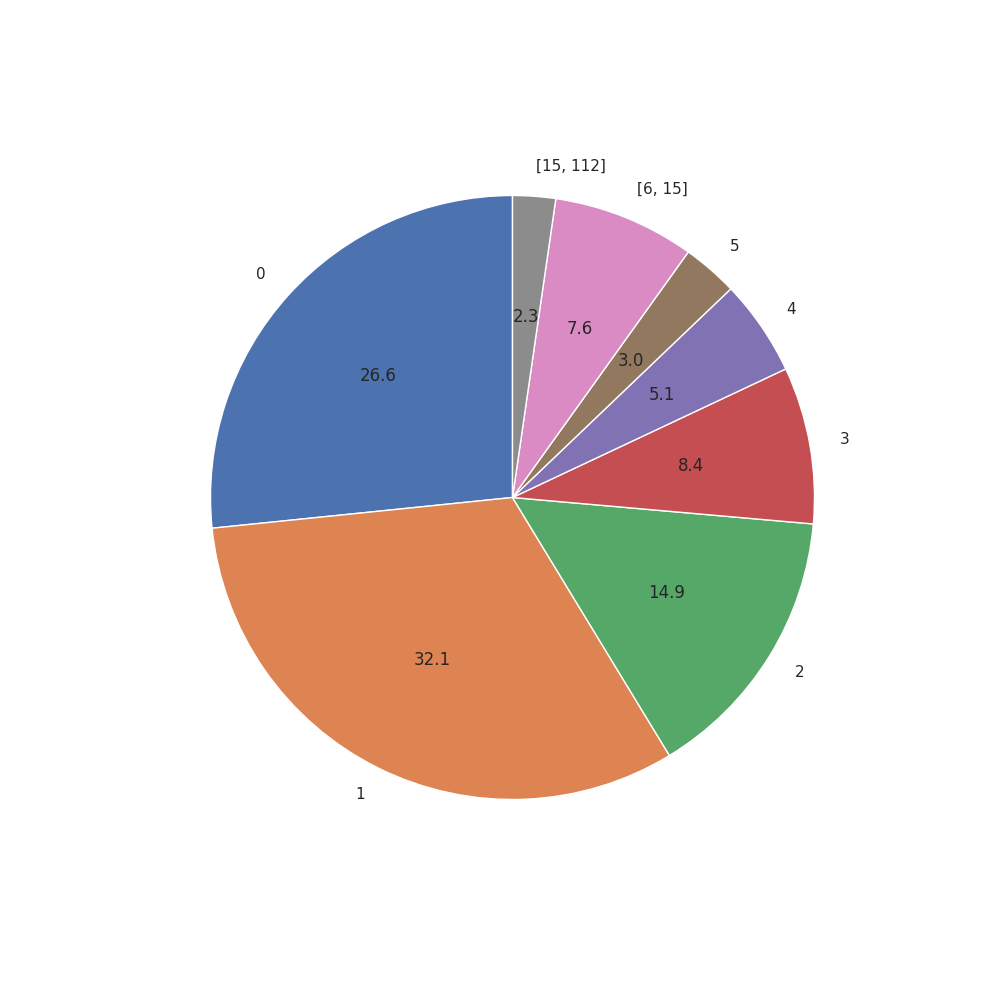
\includegraphics[width=0.32\textwidth, trim={5cm 4.7cm 4.3cm 4.6cm}, clip]{images/retinafocus_iou_90_lower}} 
        \caption{Tỷ lệ các kích thước của bounding box mà RetinaFace không dự đoán ra tương ứng với IoU 0.5 (a), IoU 0.75 (b), IoU 0.9 (c)}
        \label{fig:retinafocus_iou_lower}
    \end{figure}

    \noindent
    Cụ thể hơn, trong hình \ref{fig:retinafocus_iou_lower}, dù xét ở mức IoU nào, thì các bounding box có kích thước nhỏ từ 0 đến 60 đều chiếm tổng tỷ lệ lớn, cụ thể ... đối với IoU 0.5, ... đối với IoU 0.75 và ... đối với IoU 0.9.

    \noindent
    Hơn nữa, với kiến trúc của FPN như hình \ref{fig:retinafocus_architecture}, một bounding box có kích thước 4x4 ở ảnh đầu vào sẽ có tương ứng một khu vực có kích thước 2x2 ở feature maps ${C}_{2}$ và ${P}_{2}$, 1x1 ở feature maps ${C}_{3}$ và ${P}_{3}$ và gần như không còn thông tin ở các feature maps từ ${C}_{4}$ và ${P}_{4}$ trở đi.
    Điều này khiến cho các bounding box này trở thành các điểm dữ liệu nhiễu của nhánh Focus, khiến cho việc học của nhánh Focus bị giảm hiệu quả.

    \noindent
    Từ những phân tích trên, chúng tôi lựa chọn lần lượt các tham số $a = 5, b = 60, c = 150$ tương ứng với groundtruth bounding box có kích thước từ $5 \times 5$ đến $60 \times 60$ là các bounding box cần được focus, các groundtruth bounding box có kích thước dưới $5 \times 5$ hoặc từ $60 \times 60$ đến $150 \times 150$ là các bounding box không cần quan tâm và các groundtruth bounding box có kích thước trên $150 \times 150$ là các bounding box không cần được focus.
}